\documentclass[11pt]{beamer}
\usepackage[T1]{fontenc}
\usepackage[utf8]{inputenc}
\usepackage{lmodern}
\usepackage[czech]{babel}
\usepackage{graphicx}
\usepackage{booktabs}
\usepackage{multirow}
\usepackage{amsmath}
\usepackage{array}
\usepackage{float}
\usepackage{adjustbox}
\usepackage{tikz}
\usetikzlibrary{positioning}

\usetheme{Madrid}
\usecolortheme{default}
\definecolor{farmdarkgreen}{HTML}{174C35}
\definecolor{farmgreenmid}{HTML}{245E43}
\definecolor{farmgreenlight}{HTML}{347253}
\definecolor{farmgreenpale}{HTML}{E7F0EA}
\setbeamercolor{structure}{fg=farmdarkgreen}
\setbeamercolor{palette primary}{bg=farmdarkgreen,fg=white}
\setbeamercolor{palette secondary}{bg=farmgreenmid,fg=white}
\setbeamercolor{palette tertiary}{bg=farmgreenlight,fg=white}
\setbeamercolor{palette quaternary}{bg=farmdarkgreen,fg=white}
\setbeamercolor{title}{fg=white,bg=farmdarkgreen}
\setbeamercolor{frametitle}{fg=white,bg=farmdarkgreen}
\setbeamercolor{block title}{fg=white,bg=farmdarkgreen}
\setbeamercolor{block body}{fg=black,bg=farmgreenpale}
\setbeamertemplate{navigation symbols}{}
\setbeamertemplate{caption}[numbered]
\setbeamerfont{title}{size=\Large}
\setbeamerfont{frametitle}{size=\large}

\title{Osevní plán 2025 (Tým B)}
\author{Návrh pro rozhodování}
\date{\today}

\begin{document}

\begin{frame}
  \titlepage%
\end{frame}

\begin{frame}{Problém a cíle projektu}
  \begin{columns}[T,onlytextwidth]
    \column{0.47\textwidth}
    \begin{block}{Zadání}
      \begin{minipage}[t][4.4cm][t]{\linewidth}
        \raggedright%
        \large
        Jak rozdělit 1 000 ha mezi 20 plodin pro rok 2025 při nejistotě cen, výnosů a nákladů?
        \normalsize
        \vspace{0.2cm}

        Plán musí zohlednit také rozpočet farmy a limit zeleniny.
      \end{minipage}
    \end{block}

    \column{0.47\textwidth}
    \begin{block}{Cíle projektu}
      \begin{minipage}[t][4.4cm][t]{\linewidth}
        \raggedright%
        \begin{itemize}
          \item Vyvážit očekávaný zisk a riziko výrazné ztráty.
          \item Porovnat plány při různé averzi k riziku.
          \item Najít odolný plán při růstu nákladů.
          \item Ověřit citlivost na rozpočet a limit zeleniny.
        \end{itemize}
      \end{minipage}
    \end{block}
  \end{columns}
\end{frame}

\begin{frame}{Použité metody}
  \textbf{Vstupní data \& Predikce:}
  \begin{itemize}
    \item Historické řady 1993–2024 (ceny, výnosy, náklady a CPI).
    \item Výběr nejlepších modelů podle out-of-sample testování (CRPS, MAE).
  \end{itemize}
  
  \vspace{0.15cm}
  \textbf{Scénáře tržeb:}
  \begin{itemize}
    \item Generováno 5 000 společných scénářů pomocí ročníkového bootstrapu (zachování závislostí mezi 20 plodinami).
  \end{itemize}
  
  \vspace{0.15cm}
  \textbf{Optimalizační model (Mean-CVaR):}
  \begin{itemize}
    \item Maximalizace očekávaného zisku s penalizací nejhorších 10\,\% scénářů:
          \[\max_x (1-\lambda)E[Z(x)] + \lambda \mathrm{CVaR}_{10}[Z(x)]\]
  \end{itemize}

  \vspace{0.15cm}
  \vspace{0.1cm}
  \textbf{Odolný plán při růstu nákladů:}
  \begin{itemize}
    \item Minimalizace nejvyšší lítosti přes čtyři scénáře nákladů (základ, růst jako 2008, 2023 a 2022), při $\lambda=0{,}5$.
  \end{itemize}
\end{frame}

\begin{frame}{Analýza a výsledky: Hlavní výsledky}
  \begin{block}{Výkonnost a riziko marží 2025}
    \small
    \begin{itemize}
      \item \textbf{Ceny \& Výnosy:} Predikce výnosů výrazně překonává naivní model, u cen je zlepšení mírné.
      \item \textbf{Variabilita marží:} Zelenina nabízí vysoký očekávaný zisk, ale i při dobrém průměru má vysokou pravděpodobnost záporné marže.
    \end{itemize}
  \end{block}

  \vspace{0.1cm}
  \begin{center}
    % Zvětšení grafu na téměř plnou šířku slajdu
    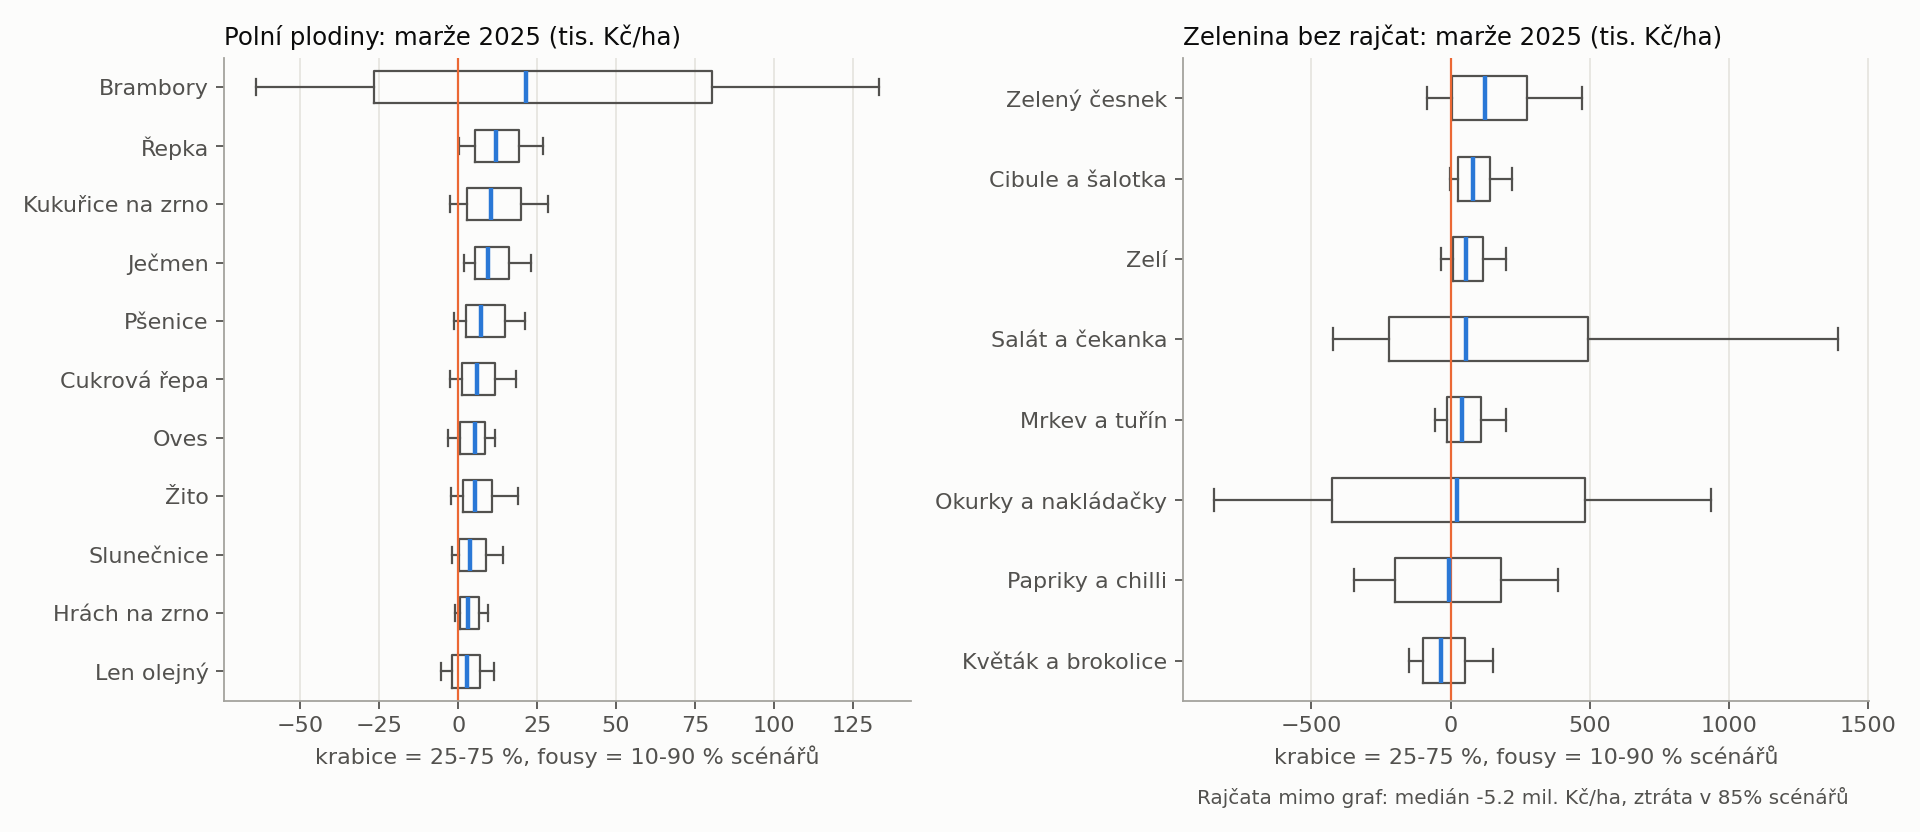
\includegraphics[width=0.90\textwidth]{vystupy/graf_marze_2025.png}
  \end{center}
\end{frame}

\begin{frame}{Citlivost na parametr $\lambda$}
  \centering
  \scriptsize
  \begin{tabular}{crrc}
    \toprule
    \textbf{$\boldsymbol{\lambda}$} & \textbf{Očekávaný zisk} & \textbf{$\boldsymbol{\mathrm{CVaR}_{\mathbf{10}}}$} & \textbf{P (ztráta)} \\
    \midrule
    0,00 & 86,9 mil. Kč & -101,0 mil. Kč & 33,5\,\% \\
    0,10 & 86,9 mil. Kč & -101,0 mil. Kč & 33,5\,\% \\
    0,25 & 76,1 mil. Kč &  -51,8 mil. Kč & 23,9\,\% \\
    0,40 & 55,6 mil. Kč &   -9,4 mil. Kč &  8,8\,\% \\
    \textbf{0,50} & \textbf{50,3 mil. Kč} & \textbf{-2,9 mil. Kč} & \textbf{5,7\,\%} \\
    0,60 & 43,1 mil. Kč &    2,8 mil. Kč &  2,7\,\% \\
    0,75 & 36,0 mil. Kč &    6,5 mil. Kč &  0,8\,\% \\
    0,90 & 33,1 mil. Kč &    7,1 mil. Kč &  0,4\,\% \\
    1,00 & 31,6 mil. Kč &    7,2 mil. Kč &  0,4\,\% \\
    \bottomrule
  \end{tabular}

  \vspace{0.3cm}
  \begin{block}{Interpretace}
    \small
    \begin{itemize}
      \item Růst $\lambda$ snižuje očekávaný zisk, ale zásadně redukuje riziko extrémních ztrát.
      \item Pro predikce jsme vybrali \textbf{$\boldsymbol{\lambda}$ = 0,5} jako referenční variantu, která nabízí vyvážený kompromis mezi očekávaným ziskem a rizikem.
    \end{itemize}
  \end{block}
\end{frame}

\begin{frame}{Vybrané plodiny pro \(\lambda=0.5\) (původní plán)}
  \begin{center}
    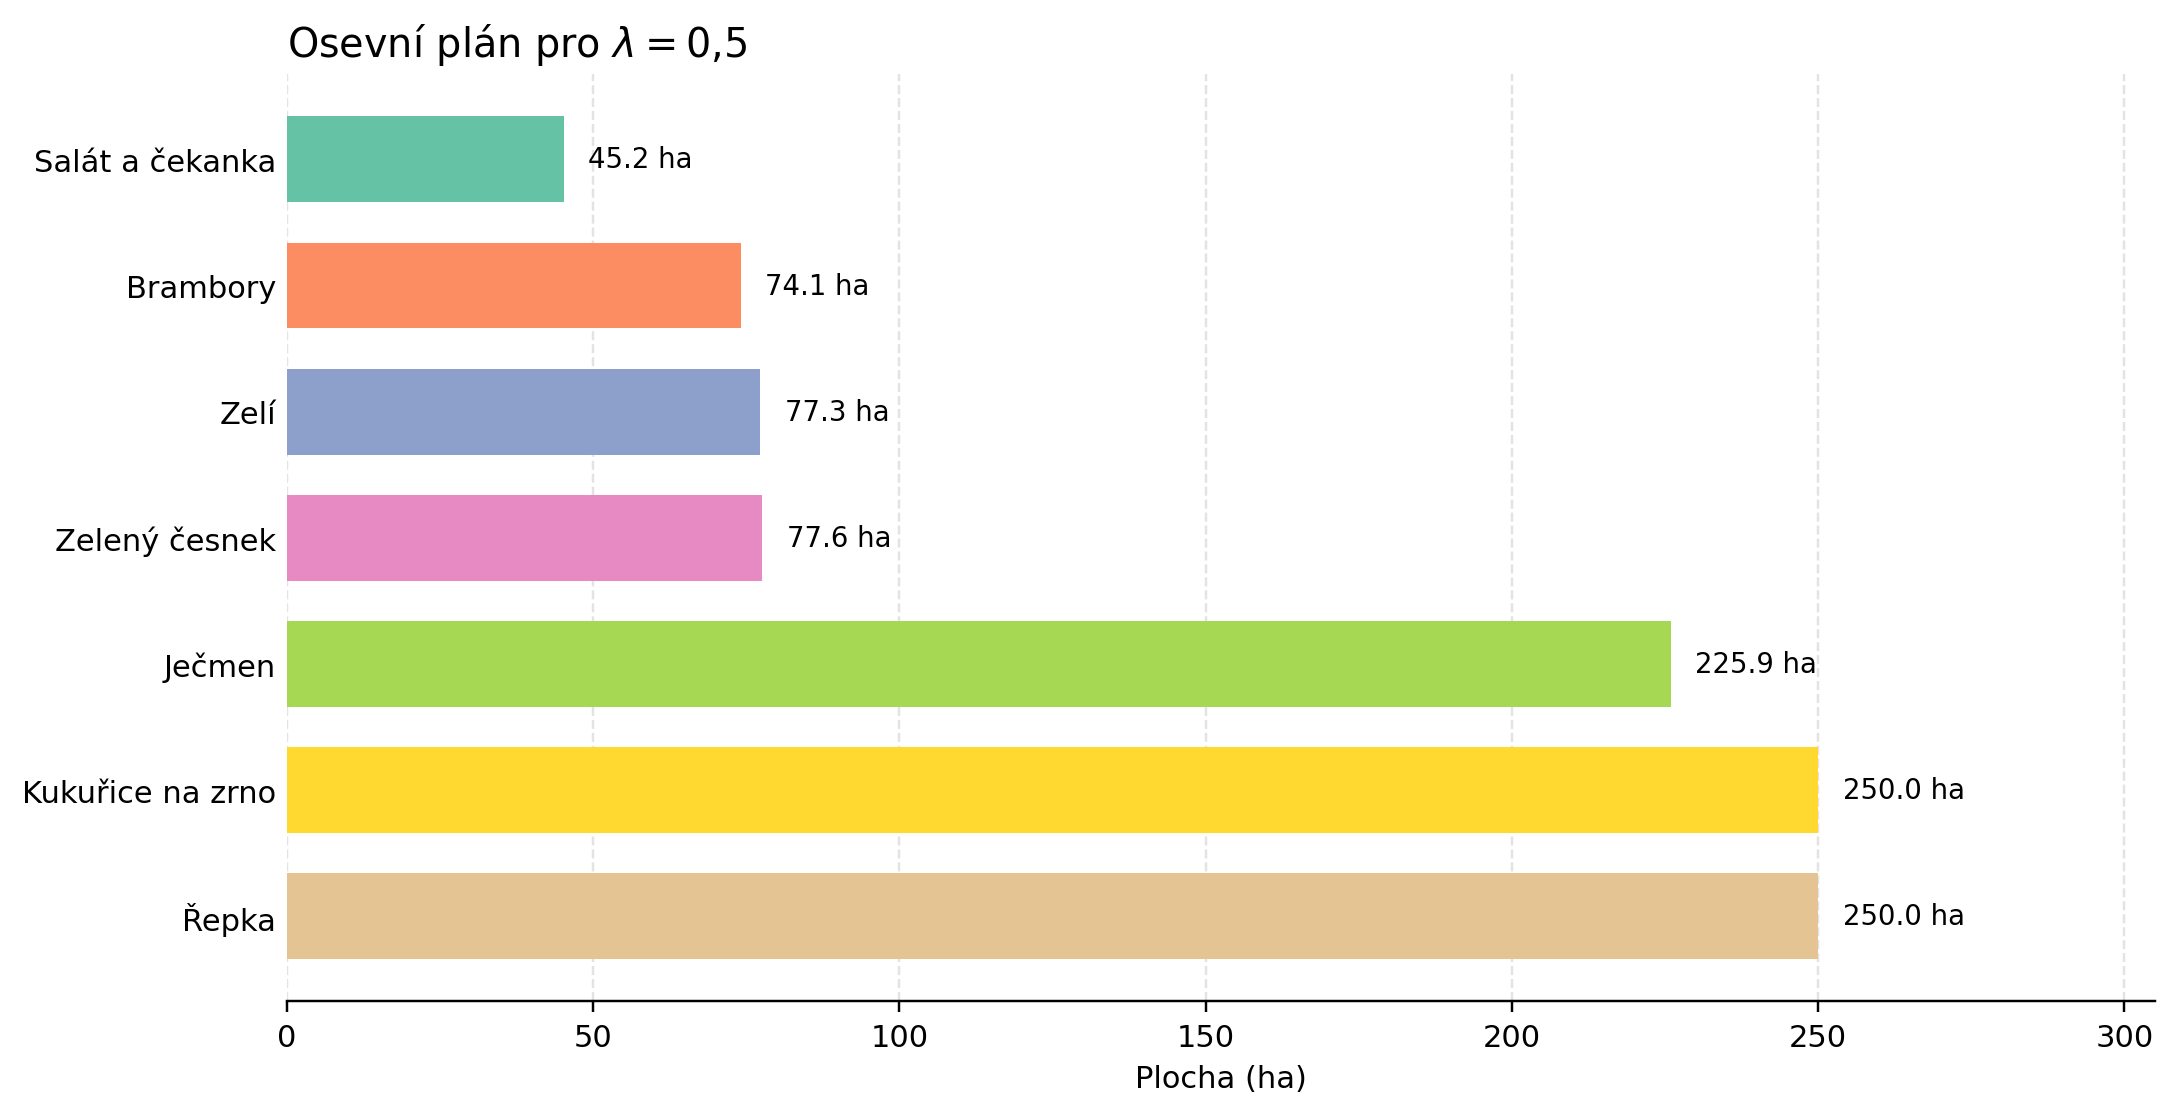
\includegraphics[width=1.0\textwidth]{vystupy/graf_plan_lambda_05_histogram.png}
  \end{center}
  \vspace{0.15cm}
  \begin{footnotesize}
    Základní plán dělí 1 000 ha mezi stabilní polní plodiny a ziskovější zeleninu (česnek, zelí, salát) s bramborami. Vyžaduje rozpočet 157 mil. Kč. Při růstu nákladů jako v roce 2022 činí očekávaný zisk 25,1 mil. Kč a riziko ztráty 25,9\%.
  \end{footnotesize}
\end{frame}

\begin{frame}{Vybrané plodiny pro \(\lambda=0.5\) (po rozšíření)}
  \begin{center}
    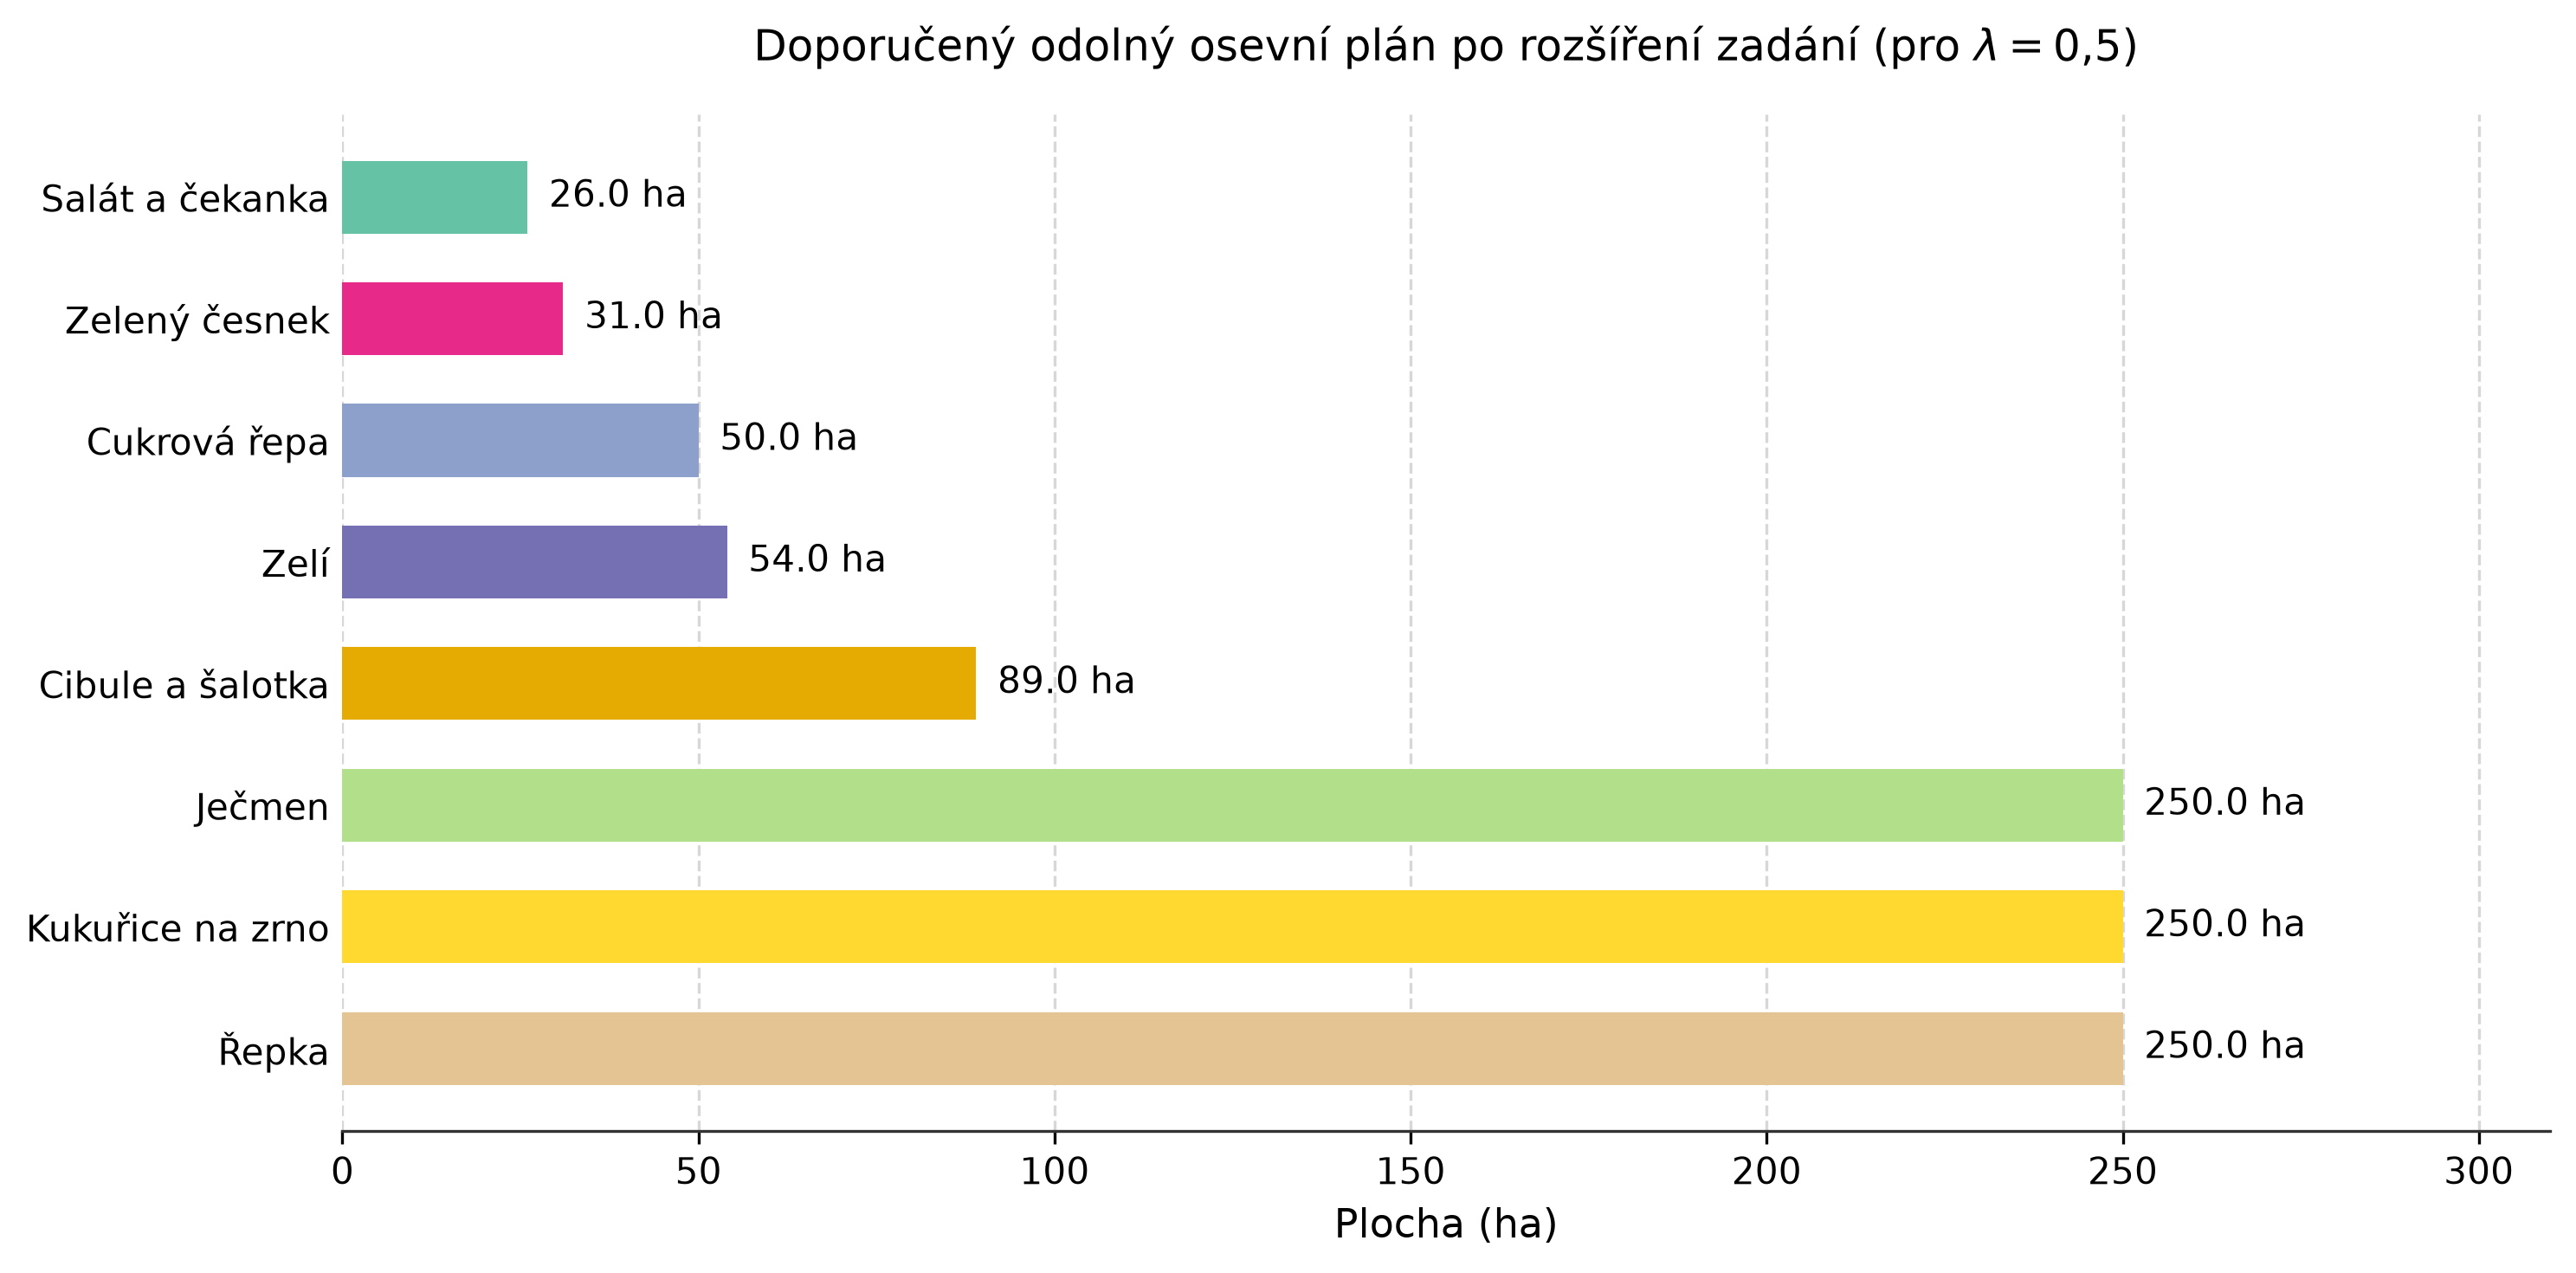
\includegraphics[width=1.0\textwidth]{vystupy/graf_odolny_plan.png}
  \end{center}
  \vspace{0.15cm}
  \begin{footnotesize}
    Odolný plán nahrazuje rizikové brambory a část česneku cibulí (89 ha) a cukrovou řepou (50 ha). Potřebuje rozpočet 110 mil. Kč (o 47 mil. Kč méně). Při růstu nákladů jako v roce 2022 dosahuje očekávaný zisk 22,3 mil. Kč a riziko ztráty klesá z 25,9\% na 15,7\%.
  \end{footnotesize}
\end{frame}

\begin{frame}{Doporučení a implikace}
  \begin{block}{Doporučení}
    \small
    \begin{itemize}
      \item Doporučujeme realizovat \textbf{Odolný osevní plán}, který šetří 47 mil. Kč v rozpočtu a výrazně snižuje riziko ztráty při zdražení vstupů.
      
      \vspace{0.2cm}
      \item Referenčně využíváme variantu \textbf{$\boldsymbol{\lambda}$ = 0,5}, vedení však může volit konzervativnější ($\lambda = 0{,}6\text{–}0{,}75$) či agresivnější přístup ($\lambda = 0{,}25\text{–}0{,}4$).
      
      \vspace{0.2cm}
      \item Před realizací doporučujeme nahradit národní agregovaná data reálnými daty farmy a ověřit skutečné kapacitní limity zeleniny.
    \end{itemize}
  \end{block}
\end{frame}

\begin{frame}{Limity analýzy}
  \begin{itemize}
    \item \textbf{Data:} Použití agregovaných národních výnosů místo farmových dat (podhodnocuje lokální rozptyl), krátká historie pozorování a omezený soubor historických extrémních událostí.
    
    \vspace{0.25cm}
    \item \textbf{Scénáře nákladů:} Ceny plodin se ve scénářích nepřizpůsobují růstu nákladů, takže reálný dopad zdražení vstupů může být mírnější.
    
    \vspace{0.25cm}
    \item \textbf{Provoz:} Kapacita zeleniny a rozpočet jsou uvažovány jako pevné tvrdé meze; model plně nezohledňuje logistiku, práci ani technické vybavení farmy.
    
    \vspace{0.25cm}
    \item \textbf{Udržitelnost:} Model nehodnotí střídání plodin, bilanci vody a živin, biodiverzitu ani celkovou pracovní náročnost.
  \end{itemize}
\end{frame}

\begin{frame}{Diskuze nad rámec zadání}
  \begin{itemize}
    \item Národní data neprokázala statisticky významné vazby, kvůli kterým by bylo nutné některé plodiny zakázat. V lokálních podmínkách farmy je však vhodné korelace dále prověřit.
    \vspace{0.35cm}
    \item Výsledný model poskytuje stabilní jádro, které lze na farmě zpřesnit o reálná data a místní podmínky.
    \vspace{0.35cm}
    \item Pro další modelování by bylo vhodné zařadit i dopad na půdu jednotlivých plodin a jejich střídání, aby se zajistila dlouhodobá udržitelnost a zdraví půdy.
  \end{itemize}
\end{frame}

\end{document}
